\section{Despliegue}

A continuación se detallan los pasos seguidos para desplegar el escenario:

\begin{enumerate}
 \item Crear tres máquinas virtuales.
 \begin{itemize}
  \item Instalar Tomcat 7 y Oracle Java 7.
  \item No hace falta configurar nada a nivel de red, tan solo saber la IP asignada en caso de modo puente, o el puerto para la traducción en modo NAT.
  \item Instalar el paquete tomcat-manager para gestionar aplicaciones con interfaz web.
 \end{itemize}
 \item Desplegar sitios web.
 \begin{itemize}
  \item Accediendo al manager de Tomcat.
  \item Se suben y despliegan los archivos .war de cada aplicacion en cada máquina virtual.
 \end{itemize}
 \item Configurar el cliente para que los nombres de dominio (descritos en la figura \ref{fig:escenario}) sean resolubles.
 \item Probar el escenario entrando en http://sp.seg.um/sp, por ejemplo. Se pueden seguir los pasos descritos en la sección \ref{sec:intercambio}.
\end{enumerate}

\begin{figure}[h!]
\centering
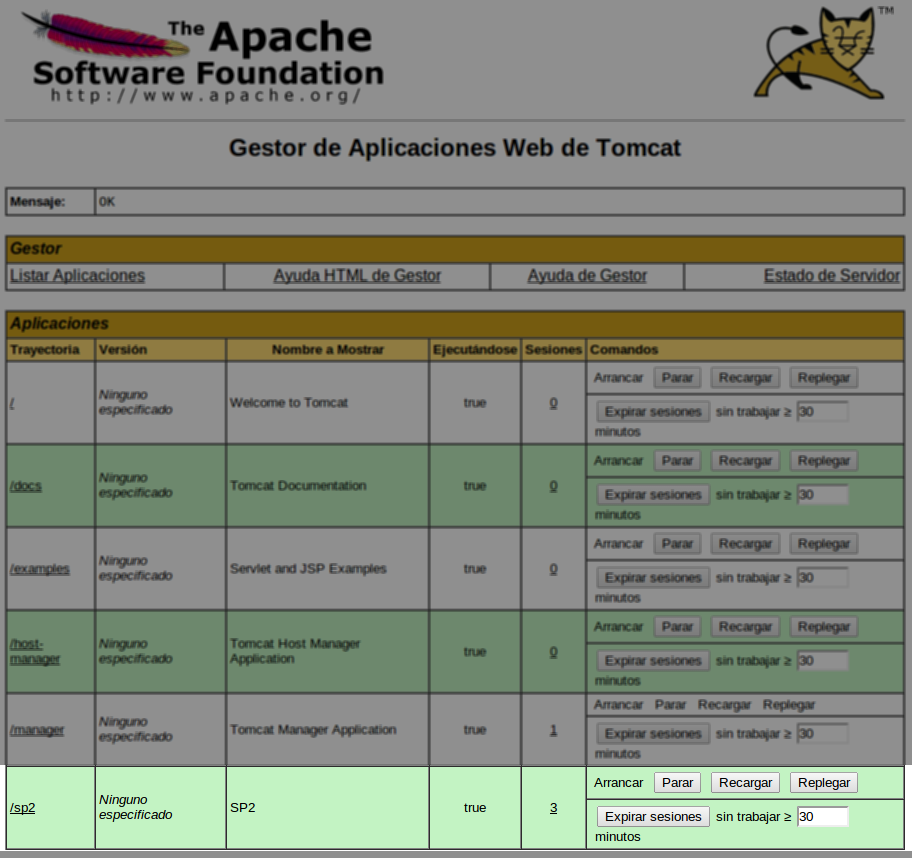
\includegraphics[width=0.9\textwidth]{img/tomcat}
\caption{Tomcat tiene desplegada la aplicacion \emph{sp2} (Service Provider 2).}
\label{fig:tomcat}
\end{figure}

El código está accesible en un repositorio público en Github: \url{https://github.com/LeandroGuillen/SAML.git}.